%%%%%%%%%%%%%%%%%%%%%%%%%%%%%%%%%%%%%%%%%%%%%%%%%%%%%%%%%%%%%%%%%%%%%%
%%%%%%%%%%%%%%%%%%%%%%%%%%%%%%%%%%%%%%%%%%%%%%%%%%%%%%%%%%%%%%%%%%%%%%
\chapter{Conventions}

\section{1d Element}
\begin{figure}[h!]
\begin{center}
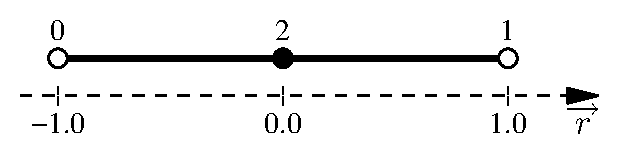
\includegraphics[width=0.4\textwidth]{figures/line}
\caption{Node numbering scheme and local coordinates for the line element}
\label{fig:conventions:1d}
\end{center}
\end{figure}

%%%%%%%%%%%%%%%%%%%%%%%%%%%%%%%%%
\newpage
\section{2d Elements}
\subsection{Quadratic Elements}

\begin{figure}[h!]
\begin{center}
\subfigure[quadratic elements]{\label{fig:conventions:quad} \includegraphics[width=0.45\textwidth]{figures/quad}}
\subfigure[triangular elements]{\label{fig:conventions:tri} \includegraphics[width=0.41\textwidth]{figures/tri}}
\caption{Node numbering scheme and surface lines. The empty nodes correpond to the quad4 element, the additional full dots to the higher order nodes of the quad8 and quad9 element.}
\label{fig:conventions:2d}
\end{center}
\end{figure}

Line pattern:
\begin{verbatim}
L0 :  0,  1,  4
L1 :  1,  2,  5
L2 :  2,  3,  6
L3 :  0,  3,  7
\end{verbatim}


\subsection{Triangular Elements}

Line pattern:
\begin{verbatim}
L0 :  0,  1,  3
L1 :  1,  2,  4
L2 :  0,  2,  5
\end{verbatim}





%%%%%%%%%%%%%%%%%%%%%%%%%%%%%%%%%%%%%%%%%%%%%%%%%%%%%%%%%%%%%%%%%%%%%%
\newpage
\section{3d}
\subsection{Hexahedral Elements}

\begin{figure}[h!]
\begin{center}
\subfigure[node pattern]{\label{fig:conventions:hex_nodes}
\includegraphics[width=0.46\textwidth]{figures/hex_nodes}}
\subfigure[surface and line pattern]{\label{fig:conventions:hex_surface_lines}
\includegraphics[width=0.43\textwidth]{figures/hex_surfaces_lines}}
\caption{Node numbering scheme and surface and lines patterns. The empty nodes correpond to the hex8 element, the additional full dots to the higher order nodes of the hex20 and hex27 element.}
\label{fig:conventions:hex}
\end{center}
\end{figure}

Surface pattern:
\begin{verbatim}
S0 :  0,  3,  2,  1, 11, 10,  9,  8, 20
S1 :  0,  1,  5,  4,  8, 13, 16, 12, 21
S2 :  1,  2,  6,  5,  9, 14, 17, 13, 22
S3 :  2,  3,  7,  6, 10, 15, 18, 14, 23
S4 :  0,  4,  7,  3, 12, 19, 15, 11, 24
S5 :  4,  5,  6,  7, 16, 17, 18, 19, 25
\end{verbatim}

Line pattern:
\begin{verbatim}
L0 :  0,  1,  8
L1 :  1,  2,  9
L2 :  2,  3, 10
L3 :  0,  3, 11
L4 :  0,  4, 12
L5 :  1,  5, 13
L6 :  2,  6, 14
L7 :  3,  7, 15
L8 :  4,  5, 16
L9 :  5,  6, 17
L10:  6,  7, 18
L11:  4,  7, 19
\end{verbatim}

\newpage
\subsection{Tetrahedral Elements}

\begin{figure}[h!]
\begin{center}
\subfigure[node pattern]{\label{fig:conventions:tet_nodes}
\includegraphics[width=0.40\textwidth]{figures/tet_nodes}}
\subfigure[surface and line pattern]{\label{fig:conventions:tet_surface_lines}
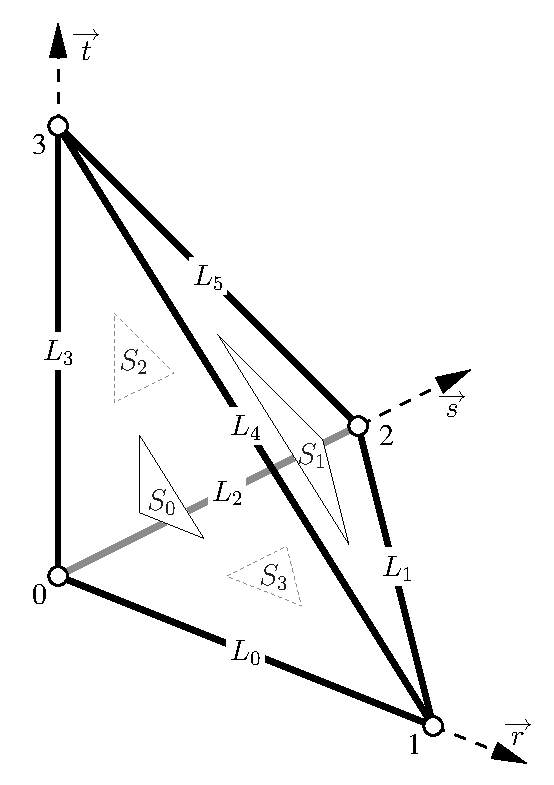
\includegraphics[width=0.41\textwidth]{figures/tet_surfaces_lines}}
\caption{Node numbering scheme and surface and lines patterns. The empty nodes correpond to the tet4 element, the additional full dots to the higher order nodes of the tet10 element.}
\label{fig:conventions:tet}
\end{center}
\end{figure}

Surface pattern:
\begin{verbatim}
S0 :  0,  1,  3,  4,  8,  7
S1 :  1,  2,  3,  5,  9,  8
S2 :  0,  3,  2,  7,  9,  6
S3 :  0,  2,  1,  6,  5,  4
\end{verbatim}

Line pattern:
\begin{verbatim}
L0 :  0,  1,  4
L1 :  1,  2,  5
L2 :  0,  2,  6
L3 :  0,  3,  7
L4 :  1,  3,  8
L5 :  2,  3,  9
\end{verbatim}





